\section{Auswertung}
\label{sec:auswertung}

Zu Beginn wurden aus den zur Vef\"ugung gestellten Datens\"atzen alle Attribute die Monte Carlo Daten, Gewichte und Labels enthalten, entfernt. Au\ss erdem wurden die Spalten entfernt, die ausschlie\ss lich den selben Wert, "Inf" oder "not a Number" enthalten.
Abschlie\ss end wurde Signal und Hintergrund Samples auf Attribute \"uberpr\"uft, die nur in einem der beiden Samples auftreten und diese ebenfalls entfernt, sodass beide Samples die selben Attribute enthalten.
Um sp\"ater zwischen Hintergrund und Signal unterscheiden zu k\"onnen, wurde an das Signal mit "0" gelabelt und der Hintergrund mit "1".

Im folgenden werden wir drei verschieden Klassifizierer auf eine Auswahl an Attributen testen. Es werden der \texttt{Naive-Bayes} Klassifizierer, der \texttt{RandomForestClassifier} und der \texttt{KNeighborsClassifier} mit Hilfe von \texttt{sklearn} verwendet.
Vorab wurden mittels der \texttt{SelectKBest} Methode die 20 besten Attribute ermittelt. Die G\"ute der Attribute wurde mit dem \texttt{f\_classif} ermittelt.
Diese Attribute sind der beigef\"ugten pdf des verwendeten jupyter Notebooks zu entnehmen.
Aus diesen Attributen wurden Test- und Trainingsdatens\"atze extrahiert, mit welchen die obigen Klassifizierer nun getestet werden.

Zuerst wurde der \texttt{RandomForestClassifier} verwendet. 
Dafür wurde ein Wald mit 100 B\"aumen gew\"ahlt. Alle anderen Parameter wurde mit default initialisiert.
Mit der Vorhersage des Klassifizierers wurden die Effizienz\footnote{wir haben den "accuracy score" von sklearn verwendet da es keinen anderen gab} und die Reinheit("precision") bestimmt.
Au\ss erdem wurde der Jaccard Score f\"ur unsere obige Attributsauswahl berechnet. Die Entsprechende ROC-Kurve ist Abbildung \ref{fig:roc_curves} zu entnehmen.
Die Ergebnisse stehen in Tabelle \ref{tab:results}.

F\"ur den \texttt{KNeighborsClassifier} wurden 20 Nachbarn gew\"ahlt. Auch hier wird die Vorhersage und der Jaccard Score in Tabelle \ref{tab:results} dargestellt sowie die ROC-Kurve in Abbildung \ref{fig:roc_curves}.

Zuletzt wurde der Naive-Bayes Klassifizierer, welcher dem Prinzip der bedingten Wahrscheinlichkeiten gen\"ugt, getestet.
Die Ergebnisse befinden sich wieder in Tabelle \ref{tab:results} und der Abbildung \ref{fig:roc_curves}.

% RFC accuracy score(sklearn) = 0.93425
% RFC precision score(sklearn) = 0.9224749327463928
% jaccard score, RFC: 0.8776174965100046

% for kNN:
% accuracy score(sklearn) = 0.879125
% Eff: 0.8733515799950237   score(sklearn) = 0.8737599206349206
% Purity: 0.8845766129032258
% Signifikanz: 41.853984367007584
% jaccard score, kNN: 0.7846325167037862

% naive bayes accuracy score(sklearn) = 0.797625
% naive bayes precision score(sklearn) = 0.753978494623656
% jaccard score, naive bayes: 0.6840975609756098

\begin{table}
  \centering
  \begin{tabular}{c | c c c}
    \toprule
    \text{Klassifizierer} & \text{Effizienz} & \text{Reinheit} & \text{Jaccard-Score} \\
    \midrule
    \text{RandomForest} & 0.93425 & 0.92247 & 0.87762 \\
    \text{KNeighborsClassifier} & 0.87913 & 0.87376 & 0.78463 \\
    \text{Naive-Bayes} & 0.79763 & 0.75398 & 0.68410 \\
    \bottomrule
  \end{tabular}
  \caption{Effizienz, Reinheit und Jaccard Score der drei verwendeten Klassifizierer.}
  \label{tab:results}
\end{table}

\begin{figure}
  \centering
  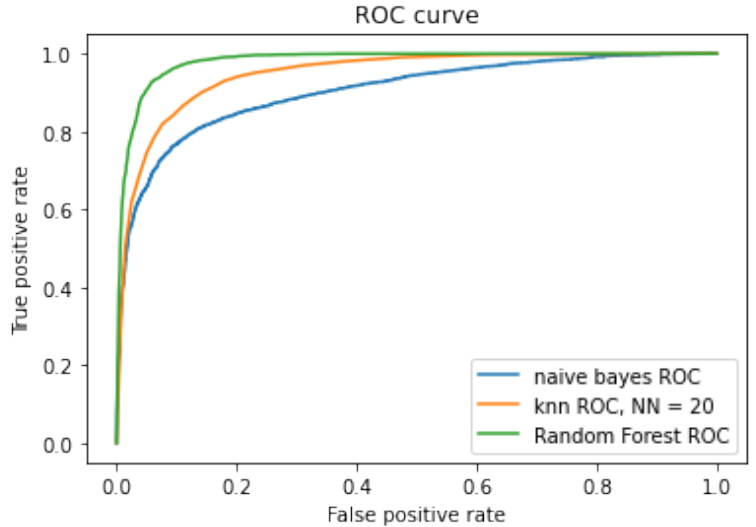
\includegraphics[width=0.8\textwidth]{plots/roc_curves.png}
  \caption{ROC-Kurven aller getesteten Klassifizierer.}
  \label{fig:roc_curves}
\end{figure}
